\documentclass{kecsmstr}
\usepackage{graphicx, epstopdf, amsmath, amssymb, color, caption, subcaption, comment, booktabs, mathabx, mathtools, varwidth, setspace, algorithm, fixltx2e}
\usepackage[algo2e, longend, noline, linesnumbered]{algorithm2e}
\SetKwIF{If}{ElseIf}{Else}{if}{then}{else if}{else}{endif}
\DeclarePairedDelimiter{\ceil}{\lceil}{\rceil}
\DeclarePairedDelimiter{\floor}{\lfloor}{\rfloor}
\DeclareMathOperator*{\argmin}{arg\,min}
\DontPrintSemicolon
\newcommand{\bE}{\mathbb{E}}
\newcommand{\bI}{\mathbb{I}}
\newcommand{\cA}{\mathcal{A}}
\newcommand{\cC}{\mathcal{C}}
\newcommand{\cD}{\mathcal{D}}
\newcommand{\cI}{\mathcal{I}}
\newcommand{\cN}{\mathcal{N}}
\newcommand{\cO}{\mathcal{O}}
\newcommand{\cS}{\mathcal{S}}
\newcommand{\cT}{\mathcal{T}}
\newcommand{\cZ}{\mathcal{Z}}
\newcommand{\eg}{{\it e.g.,}~}
\newcommand{\ie}{{\it i.e.,}~}
\newcommand{\cf}{{\it cf.}~}
\newcommand{\func}[1]{{\sc #1}}
\newcommand{\mctssr}{MCTS_{\mathcal{S}\mathcal{R}}}
\newcommand{\tuple}[1]{\ensuremath{\left \langle #1 \right \rangle }}
\newcommand{\TODO}[1]{\textbf{\color{red}#1}}
\newcommand\mycommfont[1]{\footnotesize\ttfamily{#1}}
\SetCommentSty{mycommfont}

\newcommand{\toexpand}[1]{{\it $\ll$ #1 ... $\gg$ }} 

\newcommand\NoIndent[1]{%
  \par\vbox{\parbox[t]{\linewidth}{#1}}%
}

\graphicspath{{img/}}
\DeclareGraphicsExtensions{.pdf,.jpg,.png,.eps}

\newcommand{\keywords}[1]{\par\addvspace\baselineskip
\noindent\keywordname\enspace\ignorespaces#1}

\title{Novel Selection Methods For Monte-Carlo Tree Search}
\author{Tom Pepels}

\thesistype{Master of Science of Artificial Intelligence}

\thesisdate{June 2014} \thesisnumber{14-00}

%Thesiscommittee: use \\ to separate members
\committee{Dr.~Mark~H.M. Winands\\
           Dr.~Marc~Lanctot}
% ================================

\begin{document}

% leave this in place! =============
\makeheaders \pagenumbering{roman} \maketitle \setcounter{page}{2}
\emptypage
% ================

\chapterx{Preface} 
In this thesis I present the result of my investigation into simple regret minimization for Monte-Carlo Tree Search. The thesis present the motivation, background and formal definition of a novel search algorithm based on minimizing both simple and cumulative regret. The algorithm was developed for, and tested in four two-player games: Amazons, Breakthrough, Chinese Checkers and Pentalath. The research was performed at the Department of Knowledge Engineering, Maastricht University, The Netherlands.

Special thanks goes to both Dr. Mark Winands and Dr. Marc Lanctot for providing the inspiration and guidance required to develop this novel algorithm. Their combined, vast experience was crucial to obtain the results presented in this work. Moreover, I would like to thank my wife Priscilla for her support, and for  bearing with me during the research. Without both her emotional and financial assistance you would not be reading this thesis.
\newline \newline

\noindent Tom Pepels \newline
Maastricht, May 2014
\emptypage

\chapterx{Summary} \emptypage

\tableofcontents  \emptypage 
\listofalgorithms \emptypage
\pagenumbering{arabic}

% --------------------------------------------------------------------
% ------------------- ::::::: Introduction ::::::: -------------------
% --------------------------------------------------------------------
\chapter{Introduction}

\begin{chaptercontents} An overview of Monte-Carlo Tree Search and the main topic of this thesis, simple regret minimization applied to Monte-Carlo Tree Search. Moreover, the problem statement and research questions are drafted and a general outline of the structure of the thesis is given.
\end{chaptercontents}

\section{Artificial Intelligence and Games}
Decision making and problem solving have been a core topic in Artificial Intelligence (AI) since its birth over half a century ago. In many domains an agent is required to find a specific sequence of actions to achieve a certain goal. When such a problem is defined as a graph or a tree, a search algorithm can be used to explore the state-space to find rewarding states in the future and determine the best action given the current state.
Given that most real domains are too complicated to result in a limited, specific set of rules for the agent to follow, an abstract domain is more appropriate when investigating search algorithms. For a single agent, puzzles, graph-problems and simplified real-world models are often investigated. In this case, the agent's goals are non-adversarial, it maximizes utility over time to reach a set goal. When more than one agent is involved, games provide adversarial challenges with simple rules that result in large and complex state-spaces. For most interesting games, an exhaustive search is not feasible but admissible techniques have been developed.

Even before the first computer capable of playing games at a reasonable level was developed, Alan Turing was thinking about computer chess~\citebay{turing1988chess}. Over the decades, faster computers allowed for deeper investigation into game-playing algorithms such as $\alpha\beta$~\citebay{knuth1976analysis}, Principal-Variation Search~\citebay{marsland1983relative}, Proof-number search~\citebay{allis1994proof}. One of the reasons game AI research has sparked interest over the years is that its techniques can be directly measured against human players. In 1997 {\sc Deep Blue}~\citebay{campbell2002deep} defeated then-reigning World Chess Champion Garry Kasparov in a six-game match, the first time a computer beat the human champion. After plentiful research had been performed in computer Chess, Go was the next target for game AI research. In contrary to Chess, for Go it is not straightforward to find a decent evaluation function. Moreover, in Go, over the course of the game stones can be played anywhere on the board leading to a high branching factor.

With the introduction of Monte-Carlo Tree Search~\citebay{kocsis2006bandit,coulom2007efficient}, and UCT~\citebay{kocsis2006bandit}, researchers could reach human level play in Go~\citebay{lee2010current} on small boards. Since it requires no static heuristic evaluation, using simulations to determine the rewards of states in the tree, and a selection policy to explore the tree, MCTS performed better than any algorithm had before. The success of MCTS and UCT in Go sparked researchers' interests in developing a better understanding of the algorithm and applying it to different domains ranging from games, planning problems and real-time domains~(\cf~\citeay{browne2012survey}).

\section{Monte-Carlo Tree Search}
Monte-Carlo Tree Search (MCTS) is a best-first search method based on random sampling by Monte-Carlo simulations of the state space for a specified domain~\citebay{coulom2007efficient,kocsis2006bandit}. In gameplay, this means that decisions are made based on the results of randomly simulated play-outs. MCTS has been successfully applied to various turn-based games such as Go~\citebay{lee2010current}, Lines of Action~\citebay{Winands2010b}, and Hex~\citebay{arneson2010monte}. Moreover, MCTS has been used for agents playing real-time games such as the Physical Travelling Salesman~\citebay{powleytsp}, real-time strategy games~\citebay{balla2009uct}, and Ms~Pac-Man~\citebay{realtime2014}, but also in real-life domains such as optimization, scheduling, and security~\citebay{browne2012survey}.

\begin{figure}[ht]
	\centering
	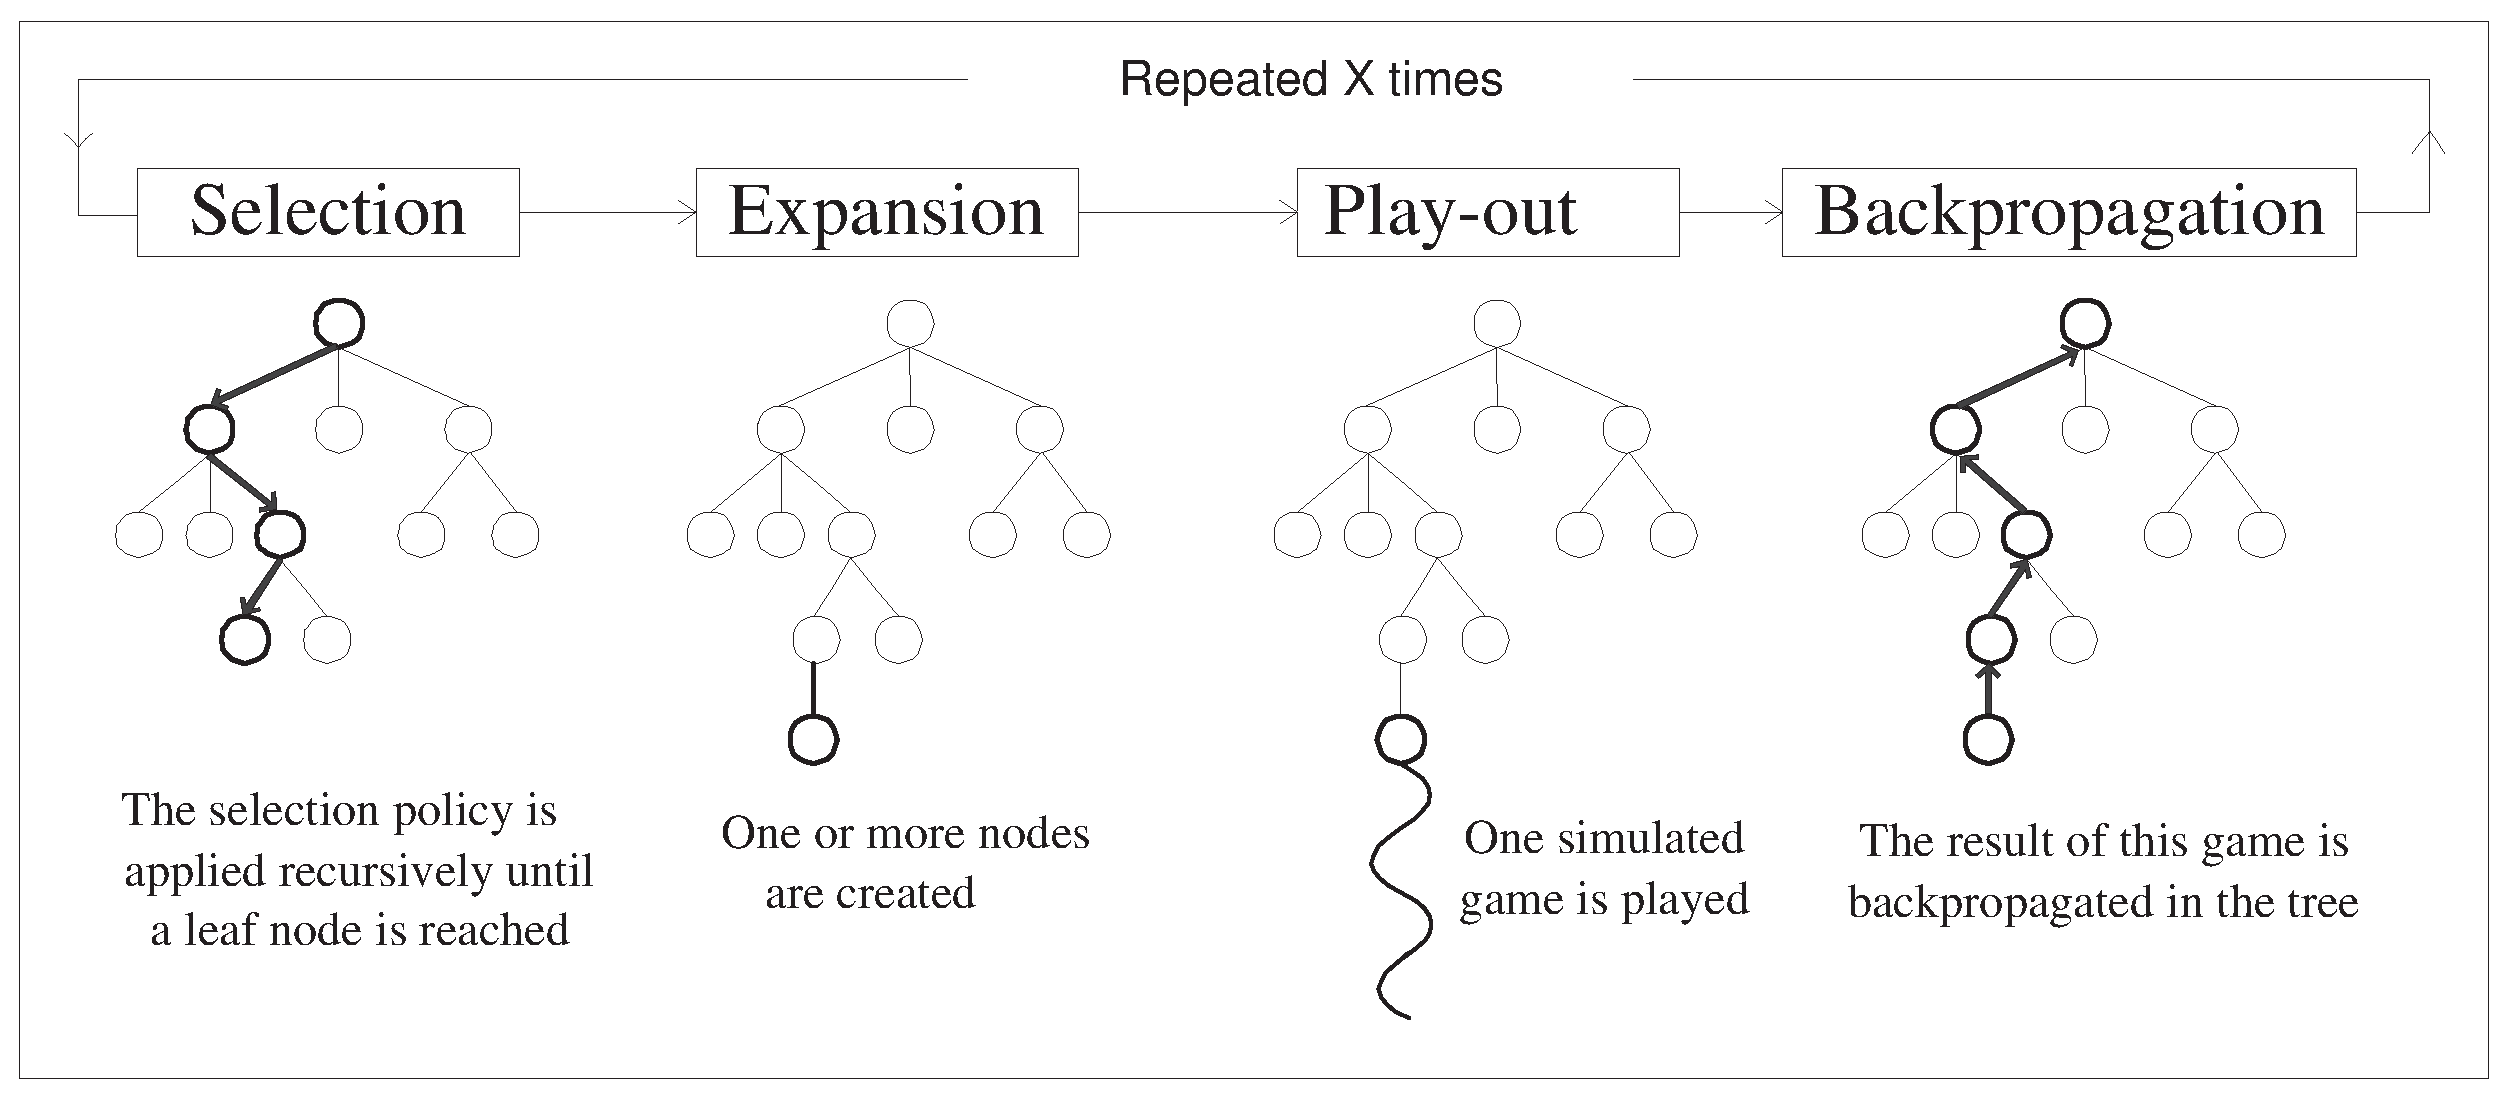
\includegraphics[width=.85\textwidth]{img/figure1.eps}
	\caption{Strategic steps of Monte-Carlo Tree Search~\protect\citebay{chaslot2008progressive}.}
	\label{fig:mcts-algorithm}
\end{figure}
\noindent In MCTS, a tree is built incrementally over time which maintains statistics at each node corresponding the rewards collected at those nodes and number of times  they have been visited. The root of this tree corresponds to the current position. The basic version of MCTS consists of four steps, which are performed iteratively until a computational threshold is reached, \ie a set number of iterations, an upper limit on memory usage, or a time constraint. The four steps at each iteration are \citebay{chaslot2008progressive}:
\begin{itemize}
\item {\bf Selection}. Starting at the root node, children are selected recursively according to a selection policy. When a leaf node is reached that does not represent a terminal state it is selected for expansion.
\item {\bf Expansion}. All children are added to the selected leaf node given available moves.
\item {\bf Play-out}. A simulated play-out is run, starting from the state of the added node. Moves are performed randomly or according to a heuristic strategy until a terminal state is reached.
\item {\bf Back-propagation}. The result of the simulated play-out is propagated immediately from the selected node back up to the root node. Statistics are updated along the tree for each node selected during the selection phase and visit counts are increased.
\end{itemize}
The combination of moves selected during the selection step, and the play-out form a single simulation. During the selection step, moves are executed according to the nodes selected in the tree, and during play-out moves are performed randomly, or according to some play-out policy.

Because results are immediately back-propagated, MCTS can be terminated any-time to determine the decision to be made. Moreover, no static heuristic evaluation is required when simulations reach an end state. However, in most cases it is beneficial to add domain knowledge for choosing moves made during the play-out.

The main benefit of MCTS is that it requires no explicit heuristic state evaluation. Rather, states are evaluated by repeatedly sampling them and measuring an average reward. That being said, it is often beneficial to add some domain knowledge to the play-outs such that the simulated games better approximate good play. Moreover, many enhancements to MCTS have been proposed to improve the general performance of the algorithm. Most notably, the MCTS-Solver \citebay{Winands2008} recognises solved wins and losses in the tree and backpropagates their values, RAVE~\citebay{gelly2007} used to speed up node valuation in the tree, and simulation-policy learning techniques such as low-level $\alpha\beta$ searches~\citebay{Winands2011}, and methods that learn a strategy online, such as the Last-Good-Reply policy~\citebay{baier2010power}, Move-average Sampling Technique (MAST)~\citebay{finnsson2008simulation}, or N-Grams~\citebay{Tak2012}. Combining these techniques often offers greatly improved play by MCTS.

\section{Regret Minimization}
The driving force behind MCTS is the notion of regret minimization. Algorithms used in multi-armed bandit (MAB) research have been developed to minimize cumulative regret. UCB~\citebay{auer2002using} is a selection policy for the MAB problem, which minimizes cumulative at a fast rate, converging to the empirically best arm fast. Once the best arm is found by exploring the available options, it exploits it by repeatedly pulling that arm, minimizing overall cumulative regret. This policy was adapted to be used in MCTS in the form of UCT~\citebay{kocsis2006bandit}

Recently, simple regret has been proposed as a new criterion for assessing the performance of both MAB~\citebay{audibert2010best,Bubeck11Pure} and MCTS~\citebay{tolpin2012mcts,Feldman12BRUE} algorithms. This is a naturally fitting quantity to optimize in the MCTS setting. All simulations executed by MCTS are for the purpose of learning good moves. However, the final move chosen after all simulations are performed, \ie the \emph{recommendation}, is the one that has real consequences. Therefore, the choice of this move should have as low as possible simple regret. Moreover, once MCTS finds a good move with high certainty, the utility of re-selecting that move diminishes over time. When a promising node, or group of nodes is visited too often, at a certain point insufficient simulation time remains to determine whether there exists a viable alternative. Rather it may be favourable to explore other options sooner, even if a single move is identified as the best. At the same time, MCTS should not `waste' its time one moves that are expected to be bad.

This is the driving idea behind full exploration algorithms such as Successive Rejects~\citebay{audibert2010best} and Sequential Halving~\citebay{Karnin13SH}. Contrary to UCB, these algorithms have no specific exploitation phase, they divide their time uniformly between a continuously reduced set of options. The final recommendation is the single arm that remains after all trials are finished.

\section{Problem Statement and Research Questions}
When MCTS is applied to games it is only the final recommendation, \ie the actual move played, that has an impact. To this end, we want the probability of selecting a suboptimal move, \ie the simple regret, to be as low as possible. Based on this assumption, simple regret minimization can be a better way to determine a move's utility. As such, an algorithm that minimizes both types of regret in their appropriate settings can improve the overall performance of MCTS. Simple regret optimization (full exploration) has practical problems, especially at low search times. Whereas algorithms based on cumulative regret perform particularly well under such limited circumstances. Given that current algorithms are either designed to minimize one type of regret, or fall short in improving performance in games. The problem statement of this thesis is:
\newline \newline
\emph{How can a Monte-Carlo Tree Search variant be constructed that minimizes both simple and cumulative regret?}
\newline \newline
The following four research questions arise from this problem statement:
\begin{enumerate}

\item{\emph{How can a search algorithm be developed for minimizing both simple and cumulative regret in a game tree?}}
\item{\emph{At which point should we switch from simple to cumulative regret minimization in the tree?}}
\newline
\NoIndent{To answer these questions, an investigation into state-of-the-art multi-armed bandit algorithms is required. Additionally, some MCTS algorithms already minimize simple regret, but have not shown general improvement in games. However, these algorithms may still prove a useful baseline.
Next, our initial assumption regarding simple regret minimization in games ought to be verified:}

\item{\emph{Will using simple regret minimizing, full exploration selection policies in MCTS improve performance in two-player games?}}
\newline
\NoIndent{This question is answered by experimentation in four different two-player games: Amazons, Breakthrough, Chinese Checkers and Pentalath. This also leads to the question whether the current foundation of MCTS research is still appropriate in the context of simple regret minimization:}
\item{\emph{Can well-known MCTS enhancements such as MCTS-Solver, Transposition Tables, Progressive History and MAST be used (more) effectively in the new algorithm?}}
\end{enumerate}

\noindent This question is crucial for the adoption of a new algorithm, because much research has been done on MCTS with UCT as its selection policy~\citebay{browne2012survey}.

\section{Thesis Outline}

The thesis opens with two introductory chapters introducing and discussing the background of the theory used. \textbf{Chapter \ref{chap:mab}}, which discusses the Multi-armed Bandit problem and its application to MCTS, and \textbf{Chapter \ref{chap:mctssr}}, in which current simple regret minimizing MCTS algorithms are discussed. The former details the exact difference between simple and cumulative regret, and how these types of regret may be minimized using different selection policies, and the latter shows how these selection policies are applied to MCTS.

Next, \textbf{Chapter \ref{chap:hybmcts}} goes into detail on Hybrid MCTS. Based on the analysis in the previous chapters, the new algorithm is defined and described. Moreover, the problems and shortcomings of the algorithm are discussed, and possible solutions provided. In \textbf{Chapter \ref{chap:experiments}} the proposed algorithm is tested in four two-player games: Amazons, Breakthrough, Chinese Checkers and Pentalath. \textbf{Chapter \ref{chap:conclusion}} concludes the thesis, and offers directions for future research and improvements.

% --------------------------------------------------------------------------------------
% ------------------- ::::::: Regret And Multi-Armed Bandits ::::::: -------------------
% --------------------------------------------------------------------------------------
\chapter{Regret And Multi-Armed Bandits}
\label{chap:mab}
\begin{chaptercontents} The foundation of regret minimization for Monte-Carlo Tree Search (MCTS) is given. Given that MCTS is a recursive multi-armed bandit algorithm, regret minimization is discussed in this context. Moreover the link between simple and cumulative regret is detailed and recent discoveries discussed.
\end{chaptercontents}

\section{Introduction}
The multi-armed bandit (MAB) problem is defined as a stochastic decision making problem~\citebay{auer2002using}. An agent is faced with several options, each with their own reward distribution. Based on empirical experimentation a decision to select the option with the best reward distribution. Generally the problem is described as choosing between the most rewarding arm of a multi-armed slot machine found in casino's. The agent can explore by pulling an arm and observing the resulting reward. The reward is drawn from either a fixed or changing probability distribution. Each pull and the returned reward constitutes a trial. 

In the classic MAB setting, the goal is to maximize the cumulative sum of rewards, \ie winning the most money in the slot machine example. Since the agent does not know the distribution of the arms beforehand, he has to \emph{explore} the possible choices, and when a rewarding arm is found, \emph{exploit} this option to gain a high total reward. Generally, after a certain limit, \eg a time-span or number of trials, the agent must return a recommendation to determine the best arm.

The performance of the agent can be evaluated by observing the difference in the rewards obtained over time and the theoretical reward obtained by pulling only the true best arm, called \emph{cumulative regret}. Or, in the case of \emph{simple regret}, observing the difference between the recommended arm and the true best arm, after the forecaster makes its final recommendation.
\vspace{2 mm}

In this chapter the different facets of MAB are discussed and related to MCTS. In Section \ref{sec:mabprob} a formal definition of the two types of regret, and their interrelation is given. Next, Section \ref{sec:ucb} discusses the well-known UCB1 selection policy and its relation to MCTS. This is followed by a review of two recently introduced selection policies for MAB aimed at minimizing simple regret, in Section \ref{sec:pureexplmab}.

\section{Regret and The Multi-Armed Bandit Problem}
\label{sec:mabprob}
Suppose a trial is setup such that a forecaster (player or agent) has $a \in [[K]] = \{ 1, 2, \cdots , K \}$ actions which can be repeatedly sampled over $t \in [[T]] = \{ 1, 2, \cdots, T \}$ trials. At each step, the forecaster receives a utility $u(a^t) \sim D_a$ according to some underlying distribution $D_a$. Suppose further that the forecaster employs a selection policy $I(t)$ which outputs some $a$ to be sampled at time $t$, and a recommendation policy $J(T)$ which selects the best arm at $T$.

\emph{Cumulative regret} is defined to be the regret of having not sampled the best single action in hindsight, 
\begin{equation}
R_c^T = \bE \left[ \max_{a' \in [[K]]} \left\{ \sum_{t=1}^T u(a') - \sum_{t=1}^T u(I(t)) \right\} \right].
\end{equation}
In other words, the regret is accumulated over time, at each trial.

Now suppose we change the experimental setup, such that the actions chosen on trials $1, 2, \ldots, T-1$ are taken under some realistic ``simulated environment'' that represents the true online decision problem but without committing to the actions. The only \emph{real} decision is made at step $T$ after having played $T-1$ simulations. In contrast, \emph{simple regret}~\citebay{Bubeck11Pure} quantifies only the regret for the recommendation policy $J$ at time $T$,

\begin{equation}
R_s^T = \bE \left[  \max_{a' \in [[K]]} \left\{ u(a') - u(J(T)) \right\} \right].
\end{equation}

In their analysis of the links between simple and cumulative regret~\citebay{Bubeck11Pure} found that upper bounds on $R_c^T$ lead to lower bounds on $R_s^T$, and that the smaller the upper bound on $R_c^T$, the higher the lower the lower bound on $R_s^T$, regardless of the recommendation policy, \ie the smaller the cumulative regret, the larger the simple regret. As such, no policy can give an optimal guarantee on both simple and cumulative regret at the same time. In the case of a multi-armed bandit the strategy used depends on the context of the problem.

\section{UCB}
\label{sec:ucb}

\citeay{auer2002using} proposed a finite time strategy for the multi-armed bandit problem. UCB1 optimizes cumulative regret over time at an optimal logarithmic rate, without knowledge of the reward distributions. The selection policy consists of two terms, 1) the current average reward, and 2) the size of the one-sided confidence interval for the average reward. For each arm, UCB1 gives an upper bounding value, below which, the true expected reward of the arm falls with high probability. The UCB1 selection policy is outlined in Algorithm \ref{alg:ucb}.

\IncMargin{1em}
\RestyleAlgo{boxruled}
\begin{algorithm2e}[ht]
	\Indm
	\KwIn{total budget $T$, arms $K$}
	\KwOut{recommendation $J_T\in K$}
	\vspace{0.2cm}
	\Indp

	play each arm once 																				\;

	\For{t=1 \emph{\KwTo} $T$} {
		Play arm $i$ that maxmizes $\bar{x}_i + \displaystyle\sqrt{\frac{2\ln{t}}{n_i}}$ \newline
		$\bar{x}_i$ is the current average reward of arm $i$, $n_i$ is the total number of trials for arm $i$ \;
	}

	\KwRet{the element of $K$ with the highest average reward}
  \caption{UCB1~\protect\citebay{auer2002using}. \label{alg:ucb}}
\end{algorithm2e}
\DecMargin{1em}

The rate of growth of cumulative regret of UCB1 is $\ln(t)$, where $t$ is the number of simulations, which was shown to be the optimal rate by~\citebay{lai1985asymptotically}. Based on this,~\citebay{Bubeck11Pure} have shown that a recommendation policy based on such a selection policy suffers a simple regret that decreases at best at a polynomial rate. 

Later in this chapter, in Section \ref{sec:mabmcts} UCB1 is discussed in the context of MCTS. Where its adopted version UCT is widely used as the preferred selection policy.

\section{Pure Exploration in Multi-Armed Bandits}
\label{sec:pureexplmab}
Non-exploiting selection policies have been proposed to decrease simple regret at high rates. Given that UCB has an optimal rate of cumulative regret convergence, and the conflicting limits on the bounds on the regret types shown by~\citebay{Bubeck11Pure}, algorithms that have a higher rate of exploration than UCB will have better bounds on simple regret. 

Consider a uniform selection policy that selects each arm $|K|/T$ times. Assuming that there are $h$ best arms, $(|K|-h)/T$ simulations are spent on inferior arms, and $h/T$ on the best ones. In games for instance, there are often only one or two good moves to be identified, and therefore, when using uniform selection, most time is wasted on pulling sub-optimal arms. Therefore, a more efficient policy is required to ensure that inferior arms are not selected as often as arms with a high utility over time.

\IncMargin{1em}
\RestyleAlgo{boxruled}
\begin{algorithm2e}[ht]
	\Indm
	\KwIn{total budget $T$, arms $K$}
	\KwOut{recommendation $J_T\in K$}
	\vspace{0.2cm}
	\Indp
	$S_1 \gets \{1,\dots,K\}$, 
	$\widebar{log}(K) \gets \frac{1}{2} + \sum_{i=2}^{K} \frac{1}{i}$
	$n_0 \gets 0$, 																\;
	\BlankLine
	\ForEach{$k\in\{1,\dots,K-1\}$} {
		$n_k = \displaystyle\ceil[\bigg]{\frac{1}{\widebar{log}(K)} \frac{n-K}{K+1-k}}$				\;
	}
	\BlankLine
	\For{k=1 \emph{\KwTo} $|K|-1$}{
		Select each arm $i\in S_k$ $n_k - n_{k-1}$ times 						\;
		$S_{k+1} \gets$ the $|S_k|-1$ empirically best arms from $S_k$			\;
	}
	\BlankLine
	\KwRet{the single element of $S_K$}
  \caption{Successive Rejects~\protect\citebay{audibert2010best}. \label{alg:succrej}}
\end{algorithm2e}
\DecMargin{1em}

Two algorithms have been proposed to solve this problem, and provide both low bounds, and an exponential rate of decrease on simple regret. The first algorithm, Successive Rejects~\citebay{audibert2010best} works by successively removing the single worst arm from the selection. The algorithm computes a budget for each round $n_k$, during the round, each arm is selected an equal number of times. After each round, the empirically worst arm is removed from the selection and a new round started. The lengths of the rounds are computed in such a manner that a specific lower bound on simple regret is guaranteed.\TODO{Should I give the exact rate of error here?} Successive Rejects is detailed in Algorithm~\ref{alg:succrej}.

A second algorithm, Sequential Halving~\citebay{Karnin13SH} takes a similar approach. As with Successive Rejects, search time is divided into rounds, and during each round arms are pulled equally often. However, instead of removing a single arm from selection after each round, half the arms are removed each time until a single one remains. The rounds in Sequential Halving are equally distributed such that each round has the same number of trials, but with a lower number of available arms. Sequential Halving is detailed in Algorithm~\ref{alg:seqhalv}.

\IncMargin{1em}
\RestyleAlgo{boxruled}
\begin{algorithm2e}[ht]
	\Indm
	\KwIn{total budget $T$, arms $K$}
	\KwOut{recommendation $J_T\in K$}
	\vspace{0.2cm}
	\Indp
	$S_0 \gets \{1,\dots,K\}$																\;
	$B \gets \ceil{\log_2{|S|}} - 1$														\;
	\BlankLine
	\For{k=0 \emph{\KwTo} $B$}{
		sample each arm $i \in S_k$ \newline														
		$n_k = \displaystyle\floor[\bigg]{\frac{T}{|S_k|\ceil{\log_2{|S|}}}}$	\newline					
		times 																				\;
		$S_{k+1} \gets$ the $|S_k|/2$ arms from $S_k$ with the empirically best average		\;
	}
	\BlankLine
	\KwRet{the single element of $S_B$}
  \caption{Sequential Halving~\protect\citebay{Karnin13SH}. \label{alg:seqhalv}}
\end{algorithm2e}
\DecMargin{1em}

Both algorithms have shown to outperform the other in different problem settings~\citebay{Karnin13SH}. \TODO{be more specific here} Moreover, both have proven theoretical guarantees with regard to the lower bounds simple regret. Based on this it holds merit to consider these algorithms as candidate substitutes for UCT in MCTS. However, based on the analysis made by~\citebay{Bubeck11Pure} discussed in Section \ref{sec:mabprob}, any method that effectively minimizes simple regret has inferior bounds on its cumulative regret. This is important in the context of search, as it relates to the two advantages discussed in subsection \ref{sec:ucb}, which we cannot expect to hold for any of the methods discussed in this section.

\section{Relation to MCTS}
\label{sec:mabmcts}
\subsection{UCT}
In MCTS, during the selection step, a policy is required to explore the tree to decide on promising options. For this reason, the widely used Upper Confidence Bound applied to Trees (UCT)~\citebay{kocsis2006bandit} was derived from the UCB1 policy. In UCT, each node is treated as a bandit problem whose arms are the moves that lead to different child nodes. UCT balances the exploitation of rewarding nodes whilst allowing exploration of lesser visited nodes. Consider a node $p$ with children $I(p)$, then the policy determining which child $i$ to select is defined as:

\begin{equation}
\label{eq:uct}
i^* = argmax_{i \in I(p)}\left\{ v_i + C \sqrt{ \frac{\ln{n_p}}{n_i}}\right\}
\end{equation}
where $v_i$ is the score of the child $i$ based on the average result of simulations that visited it, $n_p$ and $n_i$ are the visit counts of the current node and its child, respectively. $C$ is the exploration constant to tune. UCT is applied when the visit count of a child node is above a threshold $T$. When a node's visit count is below this threshold, a child is selected at random.

Note that, UCB1 and, consequentially UCT incorporate both exploitation and exploration. As such, after a number of trials, a node that is identified as the empirical best will be selected more often at an overall logarithmic rate. In tree-search this has two direct applications:
\begin{enumerate} 

\item Whenever a promising move is found, less time is spent on suboptimal moves. Since MCTS is generally time bounded it is important to spend as much time as possible exploring the best moves. Because, by the \emph{MinMax} principle in two-player games, at each ply we expect a player to maximize the minimum gain.

\item The valuation of any node in the tree is dependent on the values back-propagated. Given that UCT spends the least possible time on suboptimal moves, any values back-propagated are based on increasingly better approximations of simulations performed deeper in the tree. In fact, given infinite time, UCT will converge to selecting only moves with the highest average values.

\end{enumerate}

\subsection{Regret in MCTS}

Based on the analysis in the previous subsection, the minimization of cumulative regret is naturally suitable to tree search, and the UCB1 selection policy can be used nearly unaltered in this setting as UCT. However, as is shown in Section \ref{sec:mabprob} there exist two contexts for the multi-armed bandit problem, also to be considered in MCTS. These are:

\begin{enumerate}

\item Each trial results in a direct reward for the agent. As such we want to minimize the number of suboptimal arms pulled in order to achieve an as high as possible reward. This relates, for example, to slot machines in a casino. Every choice made at each point in the algorithm has a direct effect on the agent's reward. In this case, the reward of the agent is inversely proportional to its \textbf{cumulative regret}.

\item The agent can perform a number of trials, without consequence, in a simulated environment. The agent is allowed $T$ trials in this fashion, after which it must make a recommendation. Based on its recommendation, the agent is rewarded. In this case, the performance of the agent is measured by the \textbf{simple regret} of its recommendation. A low simple regret implies that the recommendation is close to the actual best option.

\end{enumerate}

In most MCTS literature, UCT is used as selection policy, suggesting that the first context applies. However, the second context is a more natural fit when MCTS is used to play games. The simulations are in fact performed off-line and have no effect on the match being played. The behaviour of the agent in the domain is based solely on its recommendations. 
However, simulations in MCTS do have an immediate impact on its performance. First of all, since MCTS must make a recommendation in a finite amount of time, spending more time on sub-optimal moves decreases time available to explore those expected to have high utility.

The general performance of MCTS may be improved by applying a strategy that is focussed on minimizing simple regret fast, rather than cumulative regret, in some specific part of a search-tree. Given that simple regret is a better measure of the quality of a given decision at time $T$, and that we can apply both the aforementioned contexts to search in a specific manner. 

In the next chapter, MCTS variants designed to (partially) minimize simple regret are discussed. Subsequently, in Chapter \ref{chap:hybmcts} a new search technique is proposed that uses both simple and cumulative regret minimizing policies at appropriate segments of the MCTS tree. Using this technique, we can determine whether the assumption that, when using a recursive multi-armed bandit algorithm (\ie MCTS) in games, preferring simple over cumulative regret minimization is both practical, and improves overall performance.

% -----------------------------------------------------------------------------
% ------------------- ::::::: Simple Regret In MCTS ::::::: -------------------
% -----------------------------------------------------------------------------
\chapter{Simple Regret In MCTS}
\label{chap:mctssr}

\begin{chaptercontents} A discussion on MCTS variants using simple regret minimizing selection policies. This chapter serves as introduction and inspiration to the next in which the new search technique, which combines different selection policies, is detailed.
\end{chaptercontents}

\section{Introduction}
Since the introduction of MCTS~\citebay{kocsis2006bandit} and its subsequent adoption by games researchers~(\cf~\citeay{browne2012survey}) UCT, or some variant thereof, has become the ``default'' selection policy. Since the introduction of simple regret~\citebay{Bubeck11Pure}, more MCTS research has been performed using simple regret as the minimizing metric.

\citeaby{Feldman12BRUE} have proposed an algorithm named {\sc brue}, devoted to offering the lowest possible simple regret bounds. Rather than building a connected tree such as MCTS, {\sc brue} generates non-connected nodes based on a switching function. Although the authors mention that the algorithm is a possible replacement for UCT, no evidence is provided showing improved game-play over UCT in any well-known domains. Moreover, in \citeaby{Feldman13} {\sc brue} is extended such that it may be used in more practical domains. Importantly, the proposed {\sc brue\textsubscript{i}} can be used without specifying a fixed horizon, rather it builds a tree connected to the root incrementally. \TODO{Based on initial experimentation with {\sc brue} and {\sc brue\textsubscript{i}} in the games discussed in this thesis, no improvement was show over UCT. Based on this, the algorithm is not discussed in this chapter. Rather, the results are presented in this thesis without further analysis.}

Rather than optimizing either simple, or cumulative regret throughout the MCTS tree,~\citebay{tolpin2012mcts} propose a technique in which simple regret is minimized only at the root. As is the case with {\sc brue}, the authors developed this algorithm for solving \emph{Markov decision processes} (MDP). Nevertheless, the proposed techniques are discussed in this chapter, because their approach is a key insight leading to the development of a hybrid MCTS.

Next, SHOT~\citebay{Cazenave14SHOT}, which is an MCTS algorithm based on sequential-halving~\citebay{Karnin13SH} is discussed. This algorithm was developed by the author to provide a speed-improvement over UCT, allowing more simulations per second to be performed and thereby increasing performance in game-play. However, for the purpose of a hybrid algorithm, SHOT shows how to apply the Sequential Halving selection policy recursively.

\vspace{2 mm}
In this chapter two MCTS variants are discussed. First, in section \ref{sec:srmcts}, the so-called (SR+CR) scheme proposed by~\citebay{tolpin2012mcts} is discussed. Next, in Section \ref{sec:SHOT}, a recently introduced algorithm, SHOT~\citebay{Cazenave14SHOT} is discussed. Both algorithms form the foundation of Hybrid MCTS, which is introduced in the next chapter.

\section{MCTS Based on Simple Regret}
\label{sec:srmcts}

In~\citebay{tolpin2012mcts} the authors give the same arguments presented in Chapter \ref{chap:mab}, that when MCTS is used in a the context of search in an MDP, \emph{``it is usually only the final ``arm pull'' (the actual move selection) that collects a reward, rather than all ``arm pulls''''}~\citebay{tolpin2012mcts}. Moreover, as opposed to games, it is often not useful in domains where search is required to exploit known good actions after they have been identified. Rather, more time should be spent exploring the alternatives. The hypothesis of the article is that, since only the children of the root represent an action to be taken in the domain, a selection policy that minimizes simple regret at the root, and UCT throughout the rest of the tree, should have better performance than using only UCT.

Two selection policies with lower bounds than UCT on simple regret were constructed for the purpose of selecting nodes at the root.
\begin{enumerate}
\item $\frac{1}{2}$-greedy, a policy that selects a move at random half of the time, and the current empirical best the other half. This policy offers an exponentially decreasing simple regret.
\item ${UCB}_{\sqrt{.}}$, which is similar to UCT, however the logarithm in the numerator in the upper confidence bound is replaced by a square root.
\begin{equation}
\label{eq:uctsqrt}
i^* = argmax_{i \in I(p)}\left\{ v_i + C \sqrt{ \frac{\sqrt{n_p}}{n_i}}\right\}
\end{equation}
This selection policy has a super-polynomially decreasing simple regret.
\end{enumerate}

Next, a two-stage sampling scheme named {\sc sr+cr} uses one of the above policies at the root, and UCT in the rest of the tree. In Algorithm \ref{alg:tsmcts}, the scheme proposed by the authors is given in the context of game-play.
\IncMargin{1em}
\RestyleAlgo{boxruled}
\begin{algorithm2e}[ht]
\setstretch{1.25}
	\KwIn{node $p$, current search depth}													
	\func{srcr-mcts}(node $p$, $depth = 1$):														\;
	\Indp							
	\lIf{isLeaf($p$)}{Expand($p$)}
	\eIf{$depth = 1$} {
	select child $i$ using $\frac{1}{2}$-greedy or ${UCB}_{\sqrt{.}}$								\;
	}
	{
	select child $i$ using UCT 																		\;
	}

    \eIf{isLeaf(i)} {
    	$r \gets$ {\sc playout}$(i)$ 																\;
    	\func{update} node $i$ with $r$																\;
    }
    {
    	$r \gets$ -\func{srcr-mcts}($i$, $depth + 1$)												\;
    }	
    \func{update} node $p$ with $r$																	\;
	\Indm
    \KwRet{$r$}
  \caption{Two-stage Monte-Carlo Tree Search. \label{alg:tsmcts}}
\end{algorithm2e}
\DecMargin{1em}

The selection policies were empirically validated to have lower simple regret than UCB in multi-armed bandits. Moreover, the {\sc sr+cr} scheme was shown to have lower simple regret in the MDP sailing domain. Particularly, the scheme was more advantageous when the number of nodes at the root are higher.

Although the {\sc sr+cr} scheme and two-stage MCTS was not developed for game-play, it holds merit to attempt to replicate the favourable results presented in games. As the authors argue, only the options given at the root collect any true reward from the domain, this is the case in both MDP domains and games.

\section{Sequential Halving Applied to Trees}
\label{sec:SHOT}

% --------------------------------------------------------------
% ------------------- ::::::: H-MCTS ::::::: -------------------
% --------------------------------------------------------------
\chapter{A Hybrid MCTS}
\label{chap:hybmcts}
\begin{chaptercontents}
The main contribution of this thesis, a hybrid version of MCTS, combining both simple, and cumulative regret minimizing selection policies.
\end{chaptercontents}
\section{Introduction}
As a selection policy for MCTS, UCT minimizes cumulative regret over time throughout the tree. At internal nodes, minimizing cumulative regret ensures an expected rewarding node is visited more often. First, UCT converges to a greedy selection policy where at each iteration only the expected best node is selected. In effect the average rewards at parent nodes converge to the maximum over their children, \ie UCT converges to maximum back-propagation on a stable distribution~\citebay{kocsis2006bandit}. Secondly, UCT ensures that search time is divided efficiently, as selecting suboptimal nodes is limited by $\ln(T)$ where $T$ is the number of trials~\citebay{auer2002using,kocsis2006bandit}. These two properties are not only practical when long deliberation times are feasible, rather, it is possible to terminate UCT any-time to obtain a reasonable approximation of the utility of a decision. During search this means that at each ply and at any time, MCTS can be asked for a best response to a parent's move.

In contrast, pure exploration algorithms, designed to minimize simple regret in multi-armed bandits such as Successive Rejects~\citebay{audibert2010best} and Sequential Halving~\citebay{Karnin13SH}, discussed in Chapter~\ref{chap:mab}, explore all options without specifically exploiting the best one. This results in a lower bound on simple regret only after a total of $T$ trials have completed. As such, to be used effectively, these algorithms can not be terminated at any time, and have a lower formal guarantee on the number of suboptimal selections made. Moreover,~\citebay{Bubeck11Pure} has shown that at moderate deliberation times, a modified UCB selection policy resulted in a better bound on simple regret than algorithms designed to minimize it. Relating these findings to MCTS, and assuming that, given sufficient time, minimizing simple regret gives a lower simple regret than UCT, we may choose to use a simple regret minimizing algorithm whenever sufficient trials can be performed, and switch to UCT when the computational budget is lower.

Inspired by the analysis and discussions in Chapters \ref{chap:mab} and \ref{chap:mctssr}, a new MCTS technique is proposed named Hybrid MCTS (H-MCTS). H-MCTS initializes with an explorative depth-limited search, applying a specific simple regret minimizing policy. After reaching a certain depth, where the computational budget per node is lower, the algorithm switches to the UCT selection policy. 
\vspace{2 mm}

Section \ref{sec:hybmcts} provides an introduction and analysis of H-MCTS. Next, Section \ref{sec:hybmctssolver} details the implementation of MCTS-Solver~\citeaby{Winands2008}, designed to solve positions within the tree, for H-MCTS. Lastly, Section \ref{sec:proghist} details the implementation of two types of history heuristics for the new algorithm.

\section{Hybrid MCTS}
\label{sec:hybmcts}

\IncMargin{1em}
\RestyleAlgo{boxruled}
\begin{algorithm2e}[ht]
\setstretch{1.25}
	\KwIn{node $p$, allocated budget $budget$}
	\KwOut{tuple containing the number of play-outs, $p1$ and $p2$ wins, budget spent}
	\func{h-mcts}(node $p$, $budget$):													\;
	\Indp
	\lIf{isLeaf($p$)}{$S\gets$ \func{expand}($p$)}					
	$t_s \gets \tuple{0,0,0,0}$															\;
	$s \gets |S|$																		\;
	$b \gets \displaystyle\max{\left(1, \floor[\bigg]{\frac{p.budgetSpent + budget}{s\times\ceil{log_2{s}}}}\right)}$ \;	
	\If{$p$ is not root \textbf{and} $( s = 1$ \textbf{or} $b < B )$}{
		\For{i=0 \emph{\KwTo} budget}{
			$\tuple{v, w_1, w_2, b_{u, p}}_i \gets$ \func{uct}($p$)						\;
			\func{update} $t_s$ with $\tuple{v, w_1,w_2, b_{u, p}}_i$					\;
		}
		\KwRet{$t_s$}
	}
	$b_u \gets 0$																	\;
	$S_0 \gets S$																	\;
	\While{s $>$ 1 \textbf{and} $b_u < budget$} {
		\For{i=0 \emph{\KwTo} s}{
			$n_i \gets$ node $n$ at rank $i$ of $S_k$								\;
			$b_i \gets b - n_i.visits$												\;
			\If{$b_i > 0$} {
				\If{$i = 0$ \textbf{and} $s = 2$} {
					\tcp{Spend any left-over budget on the empirically best node}
					$b_i \gets budget - b_u - (b - n_1.visits)$						\;
				}
				$b_i \gets \min{b_i, budget - b_u}$									\;
				$\tuple{v, w_1, w_2, b_u}_i \gets$ \func{h-mcts}($p$, $b_i$)		\;
				\func{update} $n_i, b_u,$ and $t_s$ with $\tuple{v, w_1, w_2, b_{u, n_i}}_i$		\;
			}
			break if $b_u \geq budget$												\;
		}
		$s \gets \ceil{\frac{s}{2}}$												\;
		$S_{k+1} \gets$ the $s$ arms from $S_k$ with the empirically best average	\;
		$k \gets k + 1$																\;
		$b \gets b + \displaystyle\max{\left(1, \floor[\bigg]{\frac{p.budgetSpent + budget}{s\times\ceil{log_2{s}}}}\right)}$ \;	
	}
	\func{update} $p.budgetSpent$ with $b_u$										\;
	\Indm
	\KwRet{$t_s$}
  \caption{Hybrid-MCTS. \label{alg:hmcts}}
\end{algorithm2e}
\DecMargin{1em}

\section{Hybrid MCTS-Solver}
\label{sec:hybmctssolver}

\section{History Heuristics for Hybrid MCTS}
\label{sec:proghist}

% -------------------------------------------------------------------------------
% ------------------- ::::::: Experiments and Results ::::::: -------------------
% -------------------------------------------------------------------------------
\chapter{Experiments and Results}
\label{chap:experiments}
\begin{chaptercontents}
The $\mctssr$ algorithm is thoroughly evaluated in the following two-player games: Amazons, Breakthrough, Chinese Checkers and Pentalath.
\end{chaptercontents}
\section{Experimental Setup}

\section{Results}

% ------------------------------------------------------------------
% ------------------- ::::::: Conclusion ::::::: -------------------
% ------------------------------------------------------------------
\chapter{Conclusion}
\label{chap:conclusion}

\bibliography{thesis} \emptypage

\appendix

\appchapter{Algorithms}

\appchapter{Detailed results}

\chapterx{Samenvatting} \emptypage

% this can be a translation of the abstract

\end{document}
